\documentclass[11pt,letterpaper]{article}

%\usepackage{times}
%\usepackage{epsfig}
\usepackage{graphicx}
%\usepackage{amsmath}
%\usepackage{amssymb}
\usepackage{hyperref}
\usepackage{tabularx}
\usepackage[left=1in, right=1in, top=1in, bottom=1in]{geometry}
\usepackage{titling}
\usepackage{setspace}
\usepackage{sectsty}
\usepackage{tabto}
\graphicspath{{./Assignment_04_NOTEBOOK_Geidel_files/}} % adds the assets directory to the path, throw your images there
\usepackage{fancyhdr}
\pagestyle{fancy}
\fancyhf{}
\fancyheadoffset{0cm}
\renewcommand{\headrulewidth}{0pt} 
\renewcommand{\footrulewidth}{0pt}
\fancyhead[R]{\thepage}
\fancypagestyle{plain}{%
  \fancyhf{}%
  \fancyhead[R]{\thepage}%
}

\usepackage{cite}
\usepackage[sectionbib]{natbib}
\renewcommand{\refname}{}

\begin{document}
\fontfamily{ptm}\selectfont
\sectionfont{\fontsize{12}{12}\fontfamily{ptm}\selectfont}
\doublespacing
%%%%%%%%%%%%%%%%%%%%%%%%%%%%%% TITLE %%%%%%%%%%%%%%%%%%%%%%%%%%%%%%%%%%%%%%
\setlength{\droptitle}{1in} 

\title{\large{ASSIGNMENT 4: \\ NORTHWESTERN MEMORIAL HEALTHCARE AGENT \\\vspace{1.2in}}}

\author{
Kevin Geidel \\
MSDS 442: AI Agent Design \& Development \\
Northwestern University \\
May 25, 2025 \\
}

\date{}
\maketitle
\thispagestyle{empty}	
\clearpage
\setcounter{page}{1}

%%%%%%%%%%%%%%%%%%%%%%%%%%%%%% PAGE 1 %%%%%%%%%%%%%%%%%%%%%%%%%%%%%%%%%%%%

\section*{Requirements 1 and 2: Graph the agent with LangChain/LangGraph}
\tab The construction of the agent and accompanying graph begins with the creation of the elements (classes and functions) that serve as nodes and edges in our graph. This begins as early as cell 2 (see appendix) with the creation of the \texttt{InquiryState} class that tracks the current values and message history for the agent cluster.
The actual assembly of the graph itself occurs in cell 13. However the components are instantiated above that.
Following the logic in cell 13 we first instantiate an empty graph:

\begin{verbatim}
builder = StateGraph(InquiryState)
\end{verbatim}

The \texttt{builder} object has \texttt{add\_node} and \texttt{add\_edge} methods that allow us to assemble the 
components created in cells 2-12. We use \texttt{add\_conditional\_edges} to inform the graph that the next node will be determined dynamically, depending on agent/user interactions. The output is displayed graphically in cell 14 (reproduced in figure \ref{fig:graph} below.)

\begin{figure}[h!]
    \centering
    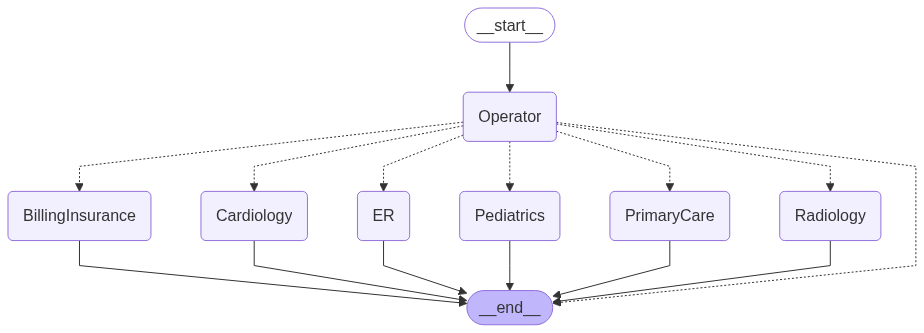
\includegraphics[width=1.0\linewidth]{Assignment_04_NOTEBOOK_Geidel_13_0.png}
    \caption{Graphical depiction of the Northwestern Memorial Healthcare Agent.}
    \label{fig:graph}
\end{figure}

We can compare the workflow in figure \ref{fig:graph} to the flowchart of desired functionality provided by Dr. Bader in the assignment requirements (figure \ref{fig:workflow}.) Each desired agent is represented as a node in the \texttt{LangGraph}. Edges represent the state being transferred from one agent to the next. 

\clearpage

\begin{figure}[h!]
    \centering
    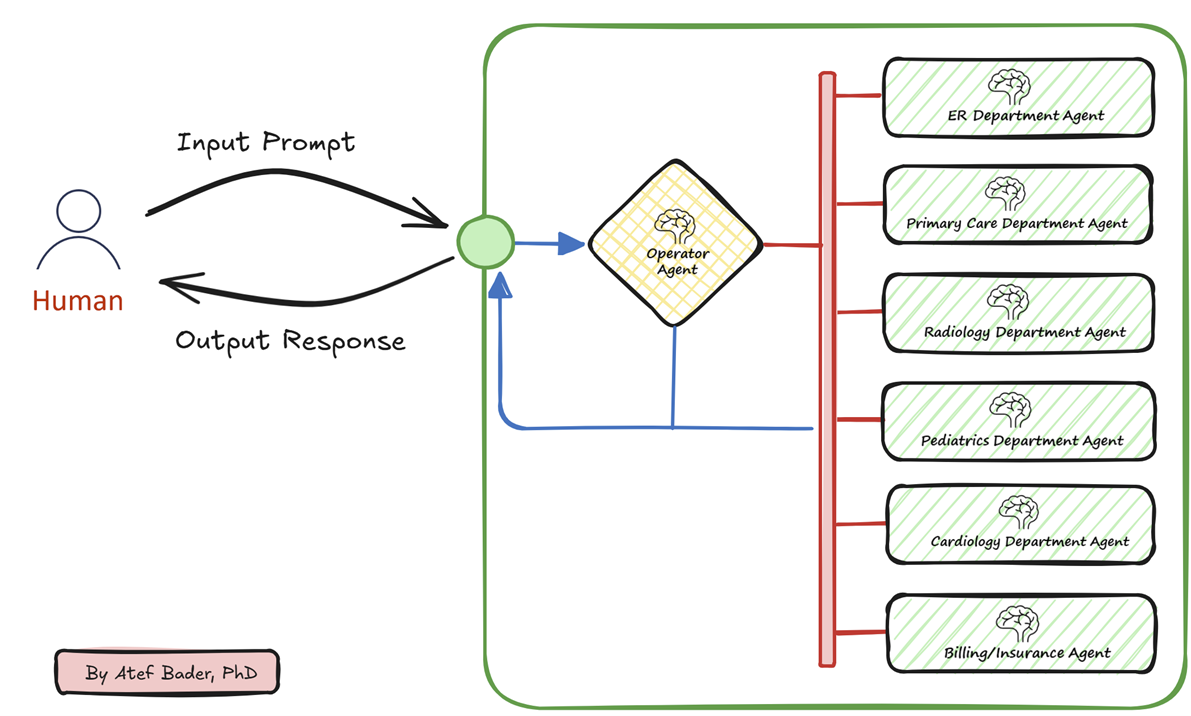
\includegraphics[width=0.7\linewidth]{target_workflow.png}
    \caption{The desired workflow as provided by the assignment objectives.}
    \label{fig:workflow}
\end{figure}


\section*{Requirement 3: The operator agent}
\tab An operator agent acts as a router to direct queries to and from the various department agents. 
The operator is constructed in cell 5 (reproduced in figure \ref{fig:operator} with line numbers.) 
Lines 2 and 3 extract the current inquiry and message history respectively. Lines 5-13 check for any termination conditions and end the conversation gracefully if present.

In order to accommodate multi-turn conversations the operator must be able to detect and respond accordingly to existing chat history.
The conditional in line 16, \texttt{if state.get('referring\_node') != "Operator" and state.get('next\_node')}, will evaluate to True if the department agents have already interacted with the user at least once (\texttt{next\_node} is not set until initially.) The five most recent messages are extracted from the state in line 17 (limit of five to avoid token overflows.) In lines 18-29 the operator invokes the LLM with a prompt crafted to evaluate the chat history and determine if the latest user query is part of an on going conversation (i.e. a follow-up question, an additional question or providing requested information.) If the LLM determines this is the case the inquiry is forwarded back to the referring node/department. This query can also decide that the latest inquiry is best served by a different department and `transfer' the inquiry to it (instead of the referring node.)

\clearpage

\begin{figure}[h!]
    \centering
    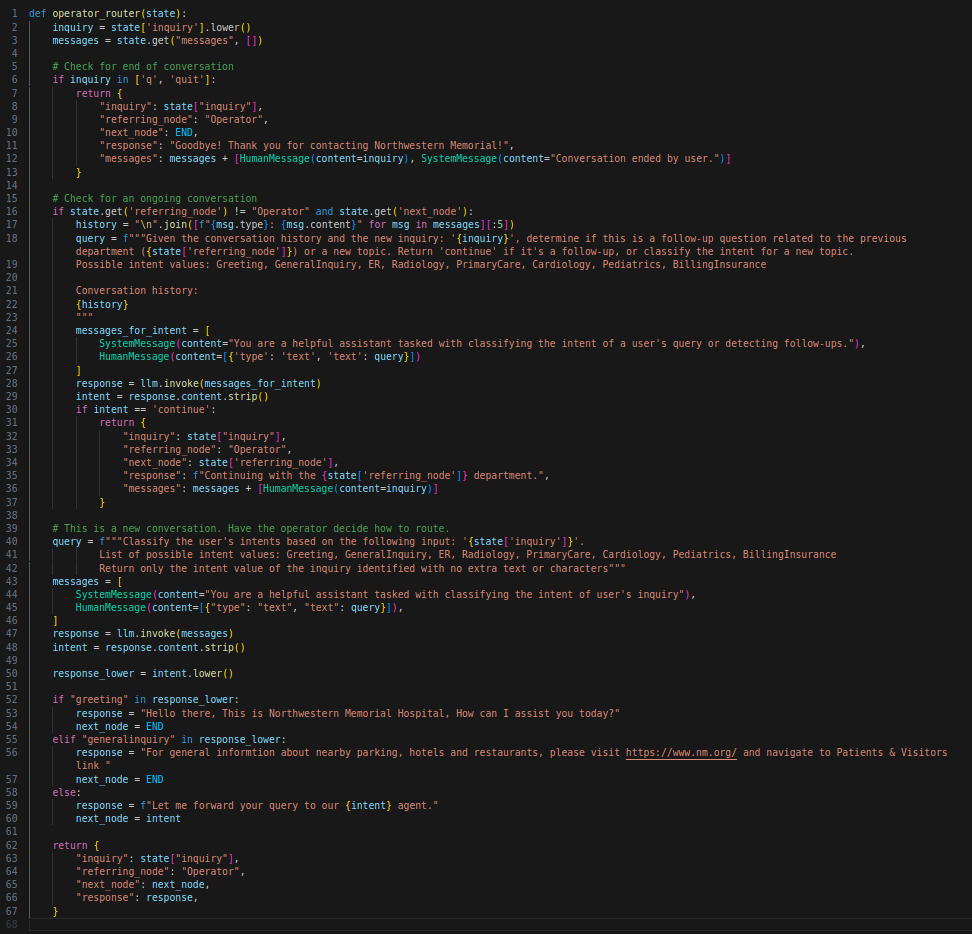
\includegraphics[width=1.0\linewidth]{cell_05.png}
    \caption{The operator/router is instantiated in cell 5.}
    \label{fig:operator}
\end{figure}

By line 39 we are on the other side of the existing conversation conditional and we can be confident that the inquiry marks a new conversation. Lines 40-50 repeat a similar query to the LLM- classifying user intent for the purposes of routing the inquiry. The difference here is there prompt does not have to consider if the inquiry is related to historic messages at all. Lines 52-57 set some hard coded responses and routes for some specific intents but, in lines 62-67, the inquiry is routed to the appropriate department specific agent.

\section*{Requirement 4: Department specific agents}
\tab Cells 7-12 instantiate functions that represent the six agents and their respective departments. 
The reader will likely note these six functions simply return the output of a common function, passed department specific arguments. The function, \texttt{department\_specific\_agent}, is an abstracted agent that performs the same steps for each department agent. These steps include loading conversation history, checking for (and reacting to) termination conditions, determining if this is an ongoing or new conversation, loading the department's knowledge base into context for new conversations, checking if the user's issue has been resolved and forwarding the state to the appropriate next node. The base department agent is defined in cell 6 and reproduced, with line numbers, in figure \ref{fig:dept_agent}.

\begin{figure}[h!]
    \centering
    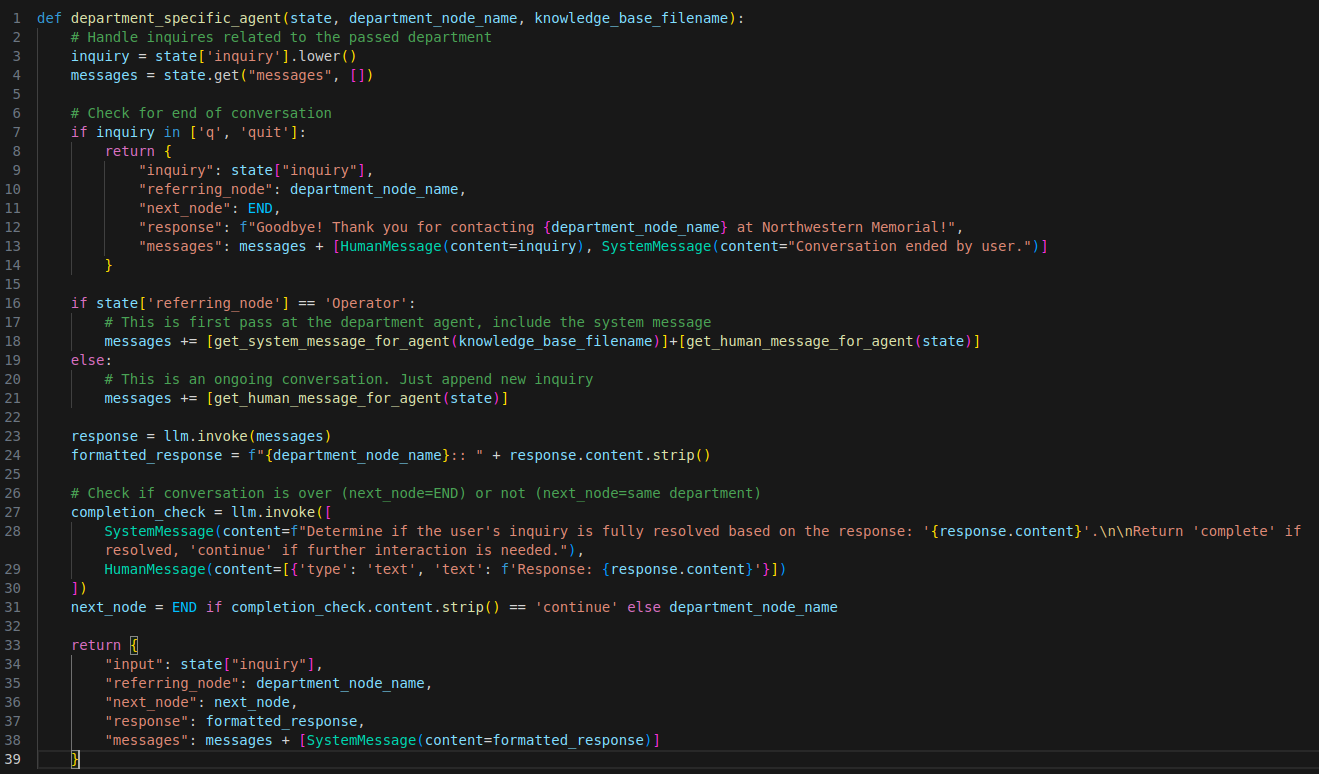
\includegraphics[width=1.0\linewidth]{cell_06.png}
    \caption{The abstracted department agent is instantiated in cell 6.}
    \label{fig:dept_agent}
\end{figure}


Lines 1-14 are similar to those of the operator- extracting what is needed from the current state and handling termination conditions (if detected.) 
This could likely be abstracted as well since the only differences related to specific hard coded messages to customize the experience (i.e. `Thank you for contacting the Cardiology Department!' vs `Come again soon!') Lines 16-21 load the latest (or first) user inquiry into messages ahead of invoking the LLM. The conditional is required to determine if the workflow has been through this department yet. If the referring node is the operator then this is the first pass through the department. The department specific \texttt{SystemMessage} (which is created dynamically from utility functions defined in cell 4) is injected into the conversation ahead of the \texttt{UserMessage}. If the referring node is this department this step is unnecessary and the current inquiry appended only.

The actual call to the LLM takes place in lines 23 and 24. Before the agent can properly route the inquiry to the next node it must first determine if the conversation is over (in which case \texttt{next\_node} is set to \texttt{END}) or if the user's request is not resolved (and \texttt{next\_node} is set back to this department.) This check is accomplished with an LLM query created in lines 27-31. The prompt is simple and asks the LLM return `continue` if the conversation is not adequately resolved. 

\section*{Requirement 5: Classifying intent}
\tab LLM queries are used to determine user intent in three different places. Two occur within the operator agent. One query is for classifying a new inquiry so that is can be routed to the appropriate department agent. This can be found in lines 40-48 of cell 5 (see figure \ref{fig:operator}.) The second query that the operator agent can use to infer user intent is for existing conversations. The LLM (lines 18-29 of cell 5 in figure \ref{fig:operator}) is tasked with deciding if the latest inquiry must go back to the referring node (to continue an ongoing conversation) or be routed to a new department.

The third instance of the agents using the LLM to classify intent happens in the respective departments. The LLM is used to decide if the conversation is over or needs to be routed back around for a multi-turn conversation. This is implemented in lines 26-31 of cell 6 (see figure \ref{fig:dept_agent}.)

\section*{Requirement 6: Knowledge base data}
\tab The agents instruct the LLM to restrict answers to the information in the department's respective knowledge base. The knowledge bases consist of six JSON files (one for each department) that contain a number of question (`inquiry') and answer (`response') entries. Some of these entries were provided with the assignment. I used Grok (\url{https://grok.com/}) to convert the provided questions and answers into the desired JSON format (figure \ref{fig:grok_formatting}.)

\clearpage

\begin{figure}[h!]
    \centering
    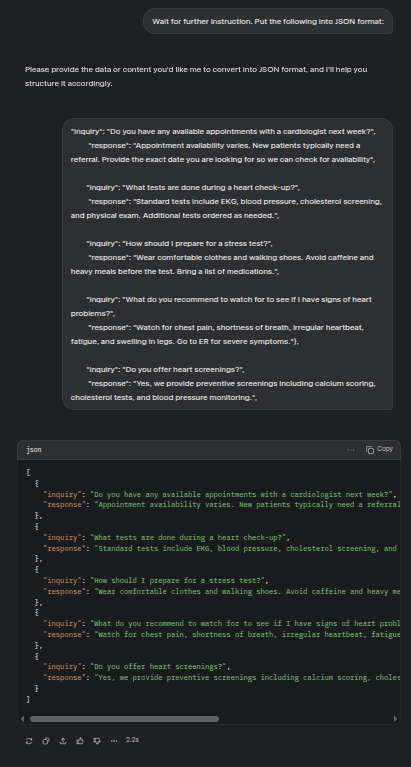
\includegraphics[height=600pt]{grok_01.png}
    \caption{The commercial AI, Grok, converting knowledge base entries into a JSON object.}
    \label{fig:grok_formatting}
\end{figure}

Grok was also used to generate new questions. Figure \ref{fig:grok_gen} shows how questions were created for the Pediatrics department and, utilizing Grok's multi-turn capability, obtaining the same JSON schema for the Emergency Department questions as well. This process was repeated until all six departments had sample data for their knowledge bases. 

\begin{figure}[h!]
    \centering
    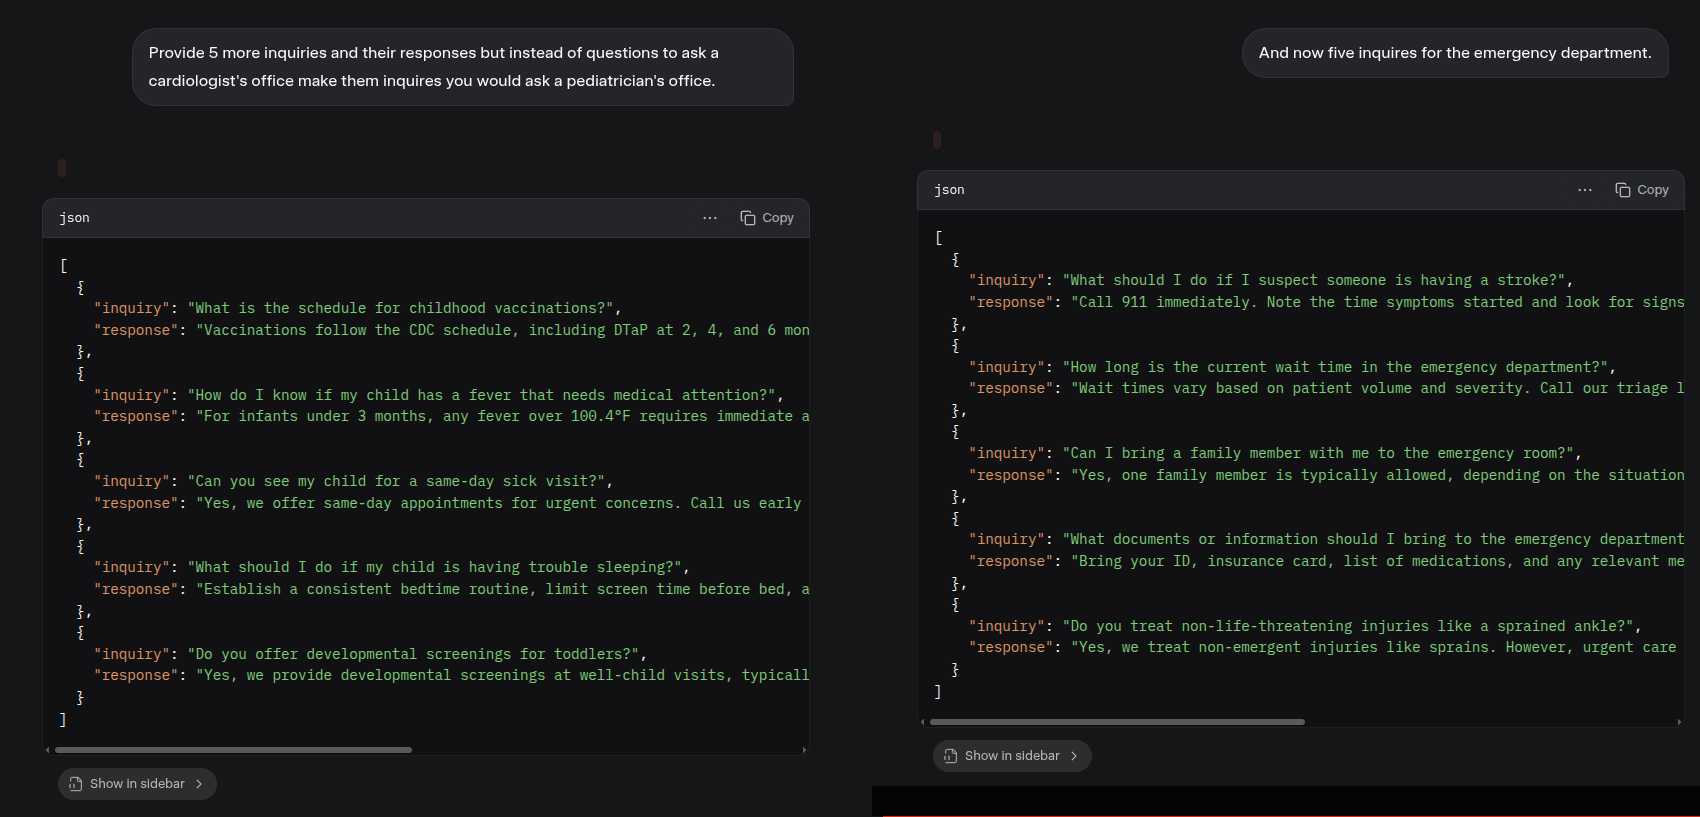
\includegraphics{grok_02.png}
    \caption{Grok was used to generate knowledge base entries in JSON format.}
    \label{fig:grok_gen}
\end{figure}

The knowledge base for a given department is loaded into context when the inquiry first arrives at that agent.
This can be seen line 18 of cell 6 (see figure \ref{fig:dept_agent}.) If the inquiry is coming from the operator the department-specific \texttt{SystemMessage} is injected into conversation history. This message is built dynamically using the \texttt{get\_system\_message\_for\_agent} utility function defined in cell 4. It uses other abstracted functions to load the proper JSON and inject it into the prompt. This is one of several ways to load documents into context. While this was simple to implement it has drawbacks. The department's knowledge base, in its entirety, is counting against our token limits (including the questions we are not using.) An improvement to this agent would be to introduce retrieval nodes that select the relevant questions from a document store in a separate step before generating the response. This would take weight off of our queries and conversation history.

\clearpage

\section*{Requirement 7: Trial runs}
\tab There are six prompts required for this assignment. All six run successfully and return expected responses (an answer based on a related knowledge base entry or a message stating no such knowledge base entry exists.) However, this does not showcase all of the features in these agents (notably, multi-turn conversations.) Because of the interactive nature of this product it is difficult to show all permutations of how to use the bot in a written report. The recorded video for this assignment contains many trials and various permutations of agent behavior. It is stored on my NU Google Drive and can be accessed here:

\noindent \url{https://drive.google.com/file/d/1IsNPPwMN7NijN8GKMiPsc1RXaHa7gqhH/view}

Cell 15 shows how the application loop is constructed. It is then utilized for one of the trial prompts. In cell 15's output we demonstrate a multi-turn conversation. Some of the inquires match knowledge base context and some do not. We can also see the completion check working when the agent acknowledges the user is done. I will conclude with the transcript (figure \ref{fig:transcript}) of one more trial, invoking several agent features.

\begin{figure}[h!]
    \centering
    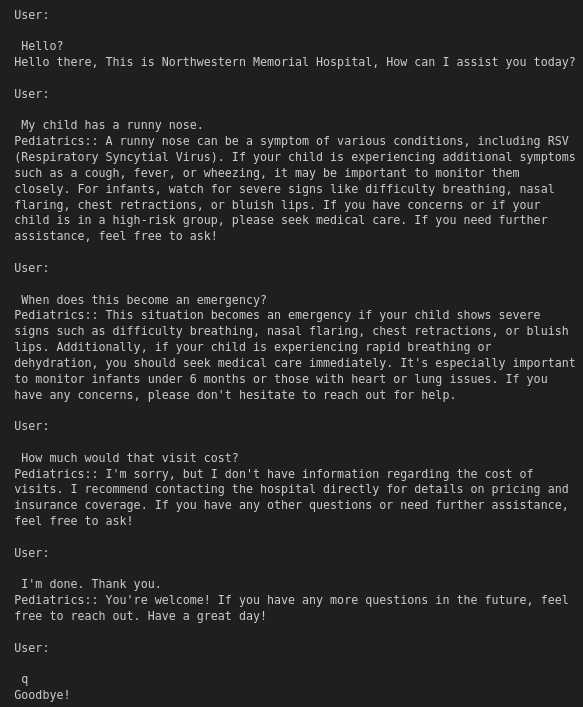
\includegraphics[height=345pt]{transcript.png}
    \caption{An example session that invokes multiple agent features.}
    \label{fig:transcript}
\end{figure}

\end{document}